% !TEX TS-program = pdflatex
% !TEX encoding = UTF-8 Unicode

% This file is a template using the "beamer" package to create slides for a talk or presentation
% - Giving a talk on some subject.
% - The talk is between 15min and 45min long.
% - Style is ornate.

% MODIFIED by Jonathan Kew, 2008-07-06
% The header comments and encoding in this file were modified for inclusion with TeXworks.
% The content is otherwise unchanged from the original distributed with the beamer package.

\documentclass{beamer}


% Copyright 2004 by Till Tantau <tantau@users.sourceforge.net>.
%
% In principle, this file can be redistributed and/or modified under

%
% However, this file is supposed to be a template to be modified
% for your own needs. For this reason, if you use this file as a
% template and not specifically distribute it as part of a another
% package/program, I grant the extra permission to freely copy and
% modify this file as you see fit and even to delete this copyright
% notice. 


\mode<presentation>
{
  \usetheme{Warsaw}
  % or ...

  \setbeamercovered{transparent}
  % or whatever (possibly just delete it)
}


\usepackage[spanish]{babel}
% or whatever

\usepackage[utf8]{inputenc}
% or whatever

\usepackage{times}
\usepackage[T1]{fontenc}
% Or whatever. Note that the encoding and the font should match. If T1
% does not look nice, try deleting the line with the fontenc.


\title[Interfaz aérea] % (optional, use only with long paper titles)
{Interfaz aérea}



\author[] % (optional, use only with lots of authors)
{W.~Bedrij\inst{1} \and F.~Benitez\inst{1} \and F.~Benitez\inst{1}}
% - Use the \inst{?} command only if the authors have different
%   affiliation.

\institute[Universities of Somewhere and Elsewhere] % (optional, but mostly needed)
{
  \inst{1}%
  Facultad de Ingeniería y Ciencias Hídricas\\
  Universidad Nacional del Litoral}
% - Use the \inst command only if there are several affiliations.
% - Keep it simple, no one is interested in your street address.

\date[Short Occasion] % (optional)
{2012}

\subject{Talks}
% This is only inserted into the PDF information catalog. Can be left
% out. 



% If you have a file called "university-logo-filename.xxx", where xxx
% is a graphic format that can be processed by latex or pdflatex,
% resp., then you can add a logo as follows:

 \pgfdeclareimage[height=0.5cm]{university-logo}{logo.png}
 \logo{\pgfuseimage{university-logo}}



% Delete this, if you do not want the table of contents to pop up at
% the beginning of each subsection:
\AtBeginSubsection[]
{
  \begin{frame}<beamer>{Presentación}
    \tableofcontents[currentsection,currentsubsection]
  \end{frame}
}


% If you wish to uncover everything in a step-wise fashion, uncomment
% the following command: 

%\beamerdefaultoverlayspecification{<+->}


\begin{document}

\begin{frame}
  \titlepage
\end{frame}

\begin{frame}{Presentación}
  \tableofcontents
  % You might wish to add the option [pausesections]
\end{frame}


% Since this a solution template for a generic talk, very little can
% be said about how it should be structured. However, the talk length
% of between 15min and 45min and the theme suggest that you stick to
% the following rules:  

% - Exactly two or three sections (other than the summary).
% - At *most* three subsections per section.
% - Talk about 30s to 2min per frame. So there should be between about
%   15 and 30 frames, all told.

\section{Introducción}

\subsection[Problema]{Problema}

\begin{frame}{PROBLEMA}{Planteo.}
  % - A title should summarize the slide in an understandable fashion
  %   for anyone how does not follow everything on the slide itself.
  	Creación de una interfaz aérea sin el uso de marcadores.
\end{frame}

\subsection[Dominio]{Dominio}
\begin{frame}{Dominio}
	Imagen capturada de una webcam.
\end{frame}


\section{Solución}

\subsection[Restricciones]{Restricciones}
\begin{frame}{RESTRICCIONES}
	\begin{itemize}
	  \item
		Brazos cubiertos
	  \item
		Evitar colores rojos en la vestimenta
	  \item
		Aparecen las manos y la cara en los fotogramas
	  \item
		No hay superposición de la mano y la cara
	\end{itemize}
\end{frame}

\subsection[Procesamiento]{Procesamiento}
\begin{frame}{PROCESAMIENTO}
   	 \begin{itemize}
   		 \item Obtención de una imagen de referencia para el fondo
   		 \item Captura de los fotogramas del vídeo
   		 \item Diferenciación con el fondo
   		 \item Enmascaramiento de la piel
   		 \item Identificación de las manos (eliminación de la cara)
   		 \item Ubicación del puntero
   	 \end{itemize}


	%\begin{figure}[tbhp]
	%\centerline{\includegraphics[scale=0.2]{varianza}}
	%\caption{Varianza de los pixeles}
	%\label{fig:varianza}
	%\end{figure}
\end{frame}


\subsection[Métodos]{Métodos}
\begin{frame}{DIFERENCIACIÓN}
		Se realiza la diferencia entre los canales RGB del frame actual contra
		la imagen de referencia del fondo.
		
		Esto permite discriminar al objeto.

	\begin{figure}[tbhp]
	\centerline{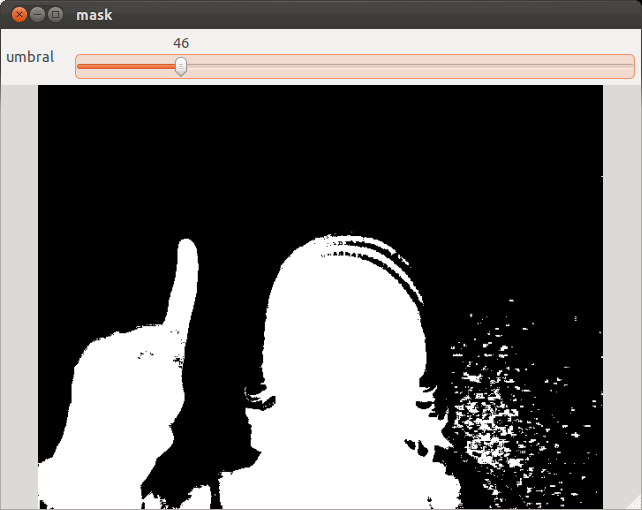
\includegraphics[scale=0.2]{3_mask}}
	\caption{Diferencia contra el fondo de referencia}
	\label{fig:diferenciacion}
	\end{figure}
\end{frame}

\begin{frame}{ENMASCARAMIENTO}
	El hue permite enmascarar la piel por umbralizado global

	Mejoras de la máscara por dilatación.

	Crecimiento inverso de regiones.
	
	$H = 7 \pm 5$ (valores experimentales de la piel)

	\begin{figure}[tbhp]
	\centerline{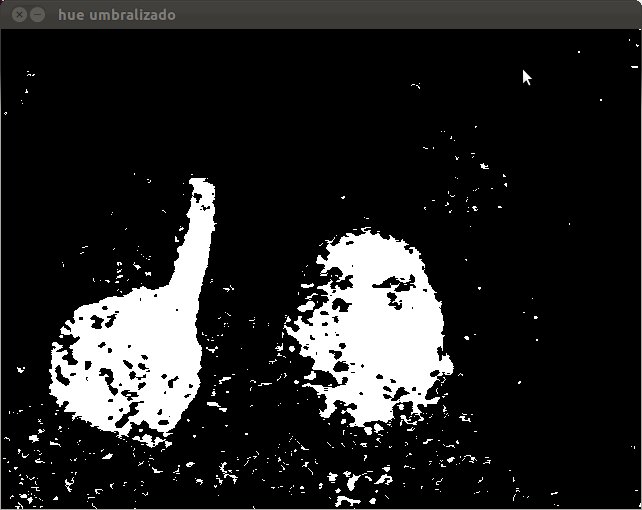
\includegraphics[scale=0.2]{2_hue_umbralizado}}
	\caption{Umbralizado del hue}
	\label{fig:hue_umbral}
	\end{figure}
\end{frame}

\begin{frame}{IDENTIFICACIÓN DE LAS MANOS}
	Heurísticas:
	\begin{itemize}
		\item Áreas.
		\item Relación aspecto (comparando contra círculo)
	\end{itemize}

	\begin{figure}[tbhp]
	\centerline{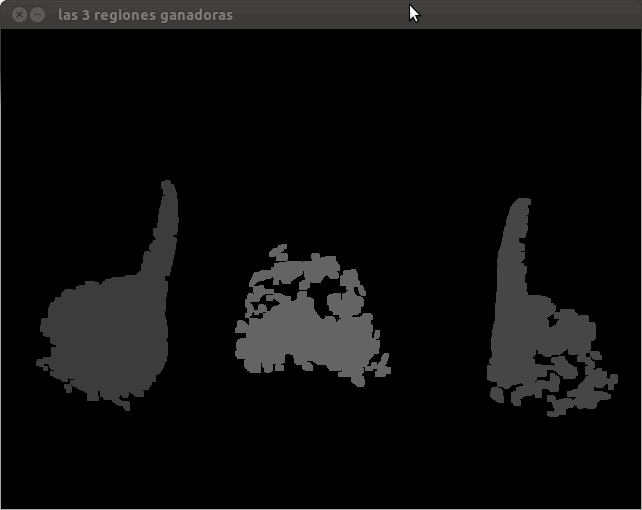
\includegraphics[scale=0.2]{5_3_regiones_ganadoras}}
	\caption{Regiones ganadoras}
	\label{fig:ganadoras}
	\end{figure}

\end{frame}

\begin{frame}{CASOS}
	\begin{itemize}
		\item Mano-mano-cara
		\item Mano-ruido-cara
	\end{itemize}

	\begin{figure}[tbhp]
	\centerline{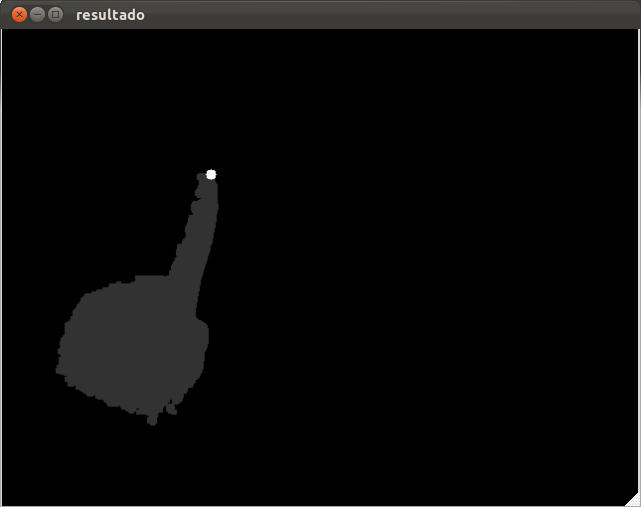
\includegraphics[scale=0.2]{6_resultado_final}}
	\caption{Casos}
	\label{fig:casos}
	\end{figure}
\end{frame}

\begin{frame}{UBICACIÓN DEL PUNTERO}
	Se utiliza el punto más alejado al centroide de la región

	\begin{figure}[tbhp]
	\centerline{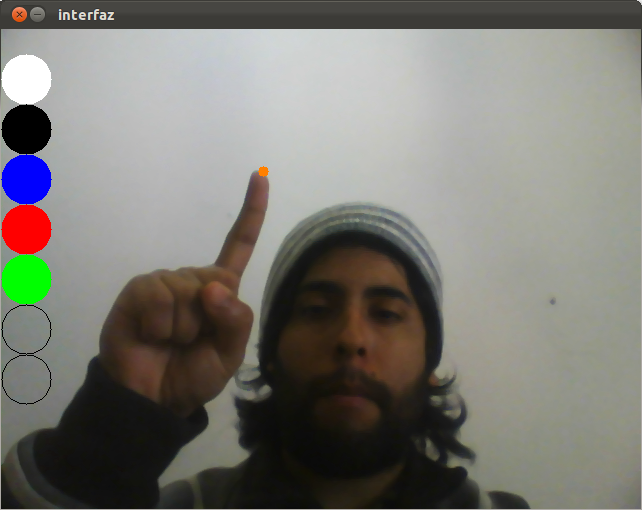
\includegraphics[scale=0.2]{7_interfaz}}
	\caption{Interfaz}
	\label{fig:7_interfaz}
	\end{figure}
\end{frame}

\section{Resultados}
	

\begin{frame}{Resultados}
La diferenciación permitió que la mano se ubicara en zonas de tonalidad parecida. 

La segmentación de la mano es crítica. Se debe evitar que aparezca como regiones separadas.

Se observan oscilaciones instantáneas producto de detecciones de puntos lejanos no deseados
\end{frame}


\section{Conclusión}
\begin{frame}{Conclusión}
		La detección de la posición de las manos fue posible en tiempo real.

		Los criterios de discriminación de las manos obligó a 
		usar una conformación en las posiciones de los dedos. 

		Para intentar solventar esos problemas, se propone realizar tracking
		de las manos, requiriendo simplemente una detección global inicial.
\end{frame}


\end{document}



